% To je predloga za poročila o domačih nalogah pri predmetih, katerih
% nosilec je Tomaž Curk. Avtor predloge je Blaž Zupan.
%
% Seveda lahko tudi dodaš kakšen nov, zanimiv in uporaben element, 
% ki ga v tej predlogi (še) ni. Več o LaTeX-u izveš na
% spletu, na primer na http://tobi.oetiker.ch/lshort/lshort.pdf.
%
% To predlogo lahko spremeniš v PDF dokument s pomočjo programa
% pdflatex, ki je del standardne instalacije LaTeX programov.

\documentclass[a4paper,11pt]{article}
\usepackage{a4wide}
\usepackage{fullpage}
\usepackage[utf8x]{inputenc}
\usepackage[slovene]{babel}
\selectlanguage{slovene}
\usepackage[toc,page]{appendix}
\usepackage[pdftex]{graphicx} % za slike
\usepackage{setspace}
\usepackage{color}
\definecolor{light-gray}{gray}{0.95}
\usepackage{listings} % za vključevanje kode
\usepackage{hyperref}
\renewcommand{\baselinestretch}{1.2} % za boljšo berljivost večji razmak
\renewcommand{\appendixpagename}{Priloge}

\lstset{ % nastavitve za izpis kode, sem lahko tudi kaj dodaš/spremeniš
	language=Python,
	basicstyle=\footnotesize,
	basicstyle=\ttfamily\footnotesize\setstretch{1},
	backgroundcolor=\color{light-gray},
}

\title{Domača naloga 3}
\author{Jernej Habjan (63150106)}
\date{\today}

\begin{document}
	
	\maketitle
	\renewcommand\thesubsection{\Alph{subsection}}

	
	\section{Uvod}
	
	Naloga je se naučiti delati z metodami nardzorovanega modeliranja, napovedovati oceno za film določenega uporabnika na podlagi ostalih uporabnikov, se poglobiti v klasifikacijo in regresiji in njune modele (Lasso, Ridge, Naivni Bayes...), primerjati smiselnost regresijske količine s klasifikacijskimi na danih podatkih.

	
	\section{Priprava podatkov}
		Izbral sem filme z več kot 100 ocenami in uporabnike, ki so ocenili več kot 100 filmov. Vendar teh je še več kot tisoč. Matrika velikosti m x n je dobro, da zgleda bolj pokončna, kar pomeni da ima več vrstic kot stolpcev, saj bomo za vsak atribut morali zgraditi svoj model, to se pravi m modelov. Zato mora biti n >> m.
		Tako sem izbral neko naključno podmnožico uporabnikov in filmov.
		Na splodnji sliki je pa predstavljena končna tabela, ki jo bom uporabljal za klasifikacijo in regresijo.
		Za stoplce imam uporabnike in njihove ocene, za vrstice pa filme in koliko ga je določeni uporabnik ocenil.
		
		\begin{figure}[!htb]
		\begin{center}
		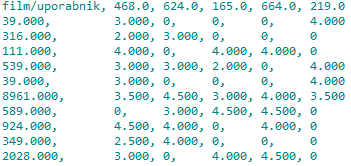
\includegraphics[scale=1.4]{slike/tabela.png}
		\caption{Pripravljena tabela na obdelavo}
		\label{slika1}
		\end{center}
		\end{figure}

		Vzel sem matriko 700 filmov in 40 uporabnikov.

	\section{Regresija}
	Prav tako kot za regresijo, je za klasifikacijo zgledal postopek nekako tako:
\begin{lstlisting}
m-krat ponovimo
  -izberemo ciljni atribut -> i-ti stolpec, in tabelo X, ki je vse ostalo
    razen ciljni atribut
  -vrstice teh dveh tabel nakljucno razdelimo tako da 75% spada v ucno,
    25% pa v testno.
  -Tako imamo 4 tabele:
    y_learn - dimenzije 75% : 1
    x_learn - dimenzije 75% : m - 1
    y_test  - dimenzije 25% : 1
    x_test  - dimenzije 25% : m - 1
  -preoblikujemo mnozico da ignorira nicle
  -naucimo model na ucni mnozici in ga testiramo na testni
  -izracunamo napako / klasifikacijsko tocnost / specificnost...
  -rezultat dodamo k ostalim rezultatom
rezultat povprecimo

\end{lstlisting}
	\subsection{Poročilo o uspešnosti}
	1. Utemeljitev mere vrednotenja:
		Izbral sem dve meri vrednotenja - MSE in Pojasnjeno varianco. MSE je dobra mera, saj lepo
		vidimo, za koliko ocen se je naš klasifikator zmotil. V tem primeru se je zmotil za približno eno
		oceno, kar je po mojem mnenju vredu.
		Prav tako ko sem pognal algoritem večkrat, je bil večinikrat algoritem Lasso boljši in znaša približno 0.7.
		
		Pri pojasnjeni varianci je pa ravno obratno. Algoritem Lasso je vračal rezultate ki so imeli manjšo napako.\\
	2. Ocenitev modelov za m uporabnikov:
		
Slika rezultatov regresije je na dnu dokumenta.

	
\begin{lstlisting}
Ocena vrednotenja MSE je: 0.935925152188
Ocena vrednotenja MSE Lasso je: 0.630111604277
Ocena vrednotenja EXPLAINED VAR je: 120.427028792
Ocena vrednotenja EXPLAINED VAR Lasso je: 5.05356984558
\end{lstlisting}	


	
	\section{Klasifikacija}
	Postopek je zelo podoben regresijskemu, vendar sem moral ocene ciljnega razreda binarizirati na oceno 0, če je ocena več ali enako 3, drugače 1.
	
	Izbral sem klasifikacijsko metodo Naivni Bayes. Njegove lastnosti:

Naivni Bayesov klasifikator je klasifikacijski model, kar pomeni, da potrebuje vrednosti iz katerih se uči, da potem lahko
pove s kolikšno verjetnostjo bi novi primer spadal v določen razred.
Te vrednosti imajo več atributov. Naivni Bayes predpostavi njihovo neodvisnost, zato lahko izračunamo naslednje enačbe:
\begin{lstlisting}
X1 = {x11, x12,...}
X2 = {...}
Y - Ciljni atribut

Bayesov obrazed: P(X,Y) = P(X|Y) * P(Y) = P(Y|X) * P(X)
Bayesov obrazec za izracun P(Y|X) -- kaksna je verjetnost filma, ce vemo oceno
P(Y|X) = (P(X|Y) * P(Y)) / P(X)

\end{lstlisting}

Manj kot je število atributov, hitreje lahko klasificiramo, ni nujno pa da bolje.



	\subsection{Poročilo o uspešnosti}
1. Utemeljitev mere vrednotenja:
Pri klasifikaciji sem vzel več mer vrednotenja:
Prva je klasifikacijska točnost. V tem primeru je bila približno 0.8 pri matriki 700 x 40.
Večinski klasifikator znaša 0.61439 kar pomeni, da je 0.8 kar dober napredek in se je model nekaj naučil.
Model ima slabo specifičnost (0.18) ampak dobro False Positive Rate (0.75).
O modelu govorim kot v povprečju m modelov, saj je za vsak stolpec svoj model - k kratno prečno preverjanje.

Prav tako imam graf (na dnu dokumenta) ROC krivulje, ki pove razmerje med True positive rate in False positive rate.
Ploščina pod grafom je nad diagonalo, ki pove da klasifikator dobro prepoznava pozitivne in negativne vrednosti.

Bolj smiselna je regresija, saj nam pove za koliko ocene se zmotimo in ne koliko ocen pravilno klasificiramo.

2. Ocenitev modelov za m uporabnikov:


\begin{lstlisting}
Mean CA: 0.802355384701, Mean ROC auc:  0.786485209927
Mean True Positive Rate: 0.1863134, Mean False Positive Rate:  0.75928382
\end{lstlisting}

Slika rezultatov klasifikacije je na dnu dokumenta.

\section{Bonus}
Izbral sem 70 naključnih najbolj popularnih filmov in jih ocenil. Ocene sem dodal kot uporabnik 9999 v tekstovno datoteko.


Za svoje filme sem napovedoval z regresijo in rezultati so naslednji (povprečeni skozi 20 iteracij):

\begin{lstlisting}
Ocena vrednotenja MSE je: 4.87814847532
Ocena vrednotenja MSE Lasso je: 2.0905359977
Ocena vrednotenja EXPLAINED VAR je: 194.890935657
Ocena vrednotenja EXPLAINED VAR Lasso je: 26.4450952912
\end{lstlisting}

Napovedal sem svoje rezultate tako, da sem 20-krat ponovil preverjanje in za y vzel uporabnika 9999.\\
Dobil sem zelo slabe rezultate. Mogoče je to zato ker sem ocenil le 70 filmov in še to nisem vseh filmov gledal. Tako da
ko sem odstranil še negledane filme, je filmov še manj.


Ko sem pogledal napovedane ocene, je nekatere ocene kar dobro ocenil, nekatere, kot pa pulp fiction pa zelo slabo.
Nekatere filme je ocenil nad 5, kar je nenavadno.

	\section{Izjava o izdelavi domače naloge}
	Domačo nalogo in pripadajoče programe sem izdelal sam.
	
	\appendix
	\appendixpage
	\section{\label{app-res}Slike}
	Slike sem priložil v mapo slike.		
	
		
	\section{\label{app-code}Programska koda}
	Programsko kodo sem zapakiral v datoteko koda.zip in jo priložil k poročilu.
	Prav tako sem v ta zip priložil datoteke potrebne za zagon programa.
	Za zagon programa odprite main.py datoteko in v funckciji main odkomentirajte funkcijo ki jo hočete testirati.



REGRESIJA:
\begin{figure}[!htb]
	\begin{center}
		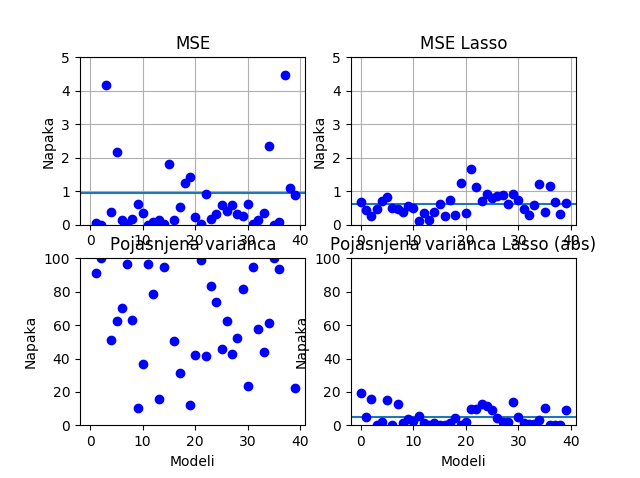
\includegraphics[scale=0.8]{slike/regresija.png}
		\caption{Levo zgoraj - Napaka MSE z algoritmom Linearna Regresija. Zgoraj desno - napaka MSE z algoritmom Lasso.
			Levo spodaj - Pojasnjena varianca z algoritmom Linearna Regresija. Spodaj desno - Pojasnjena varianca z algoritmom Lasso}
		\label{slika 2}
	\end{center}
\end{figure}


\begin{figure}[!htb]
	\begin{center}
		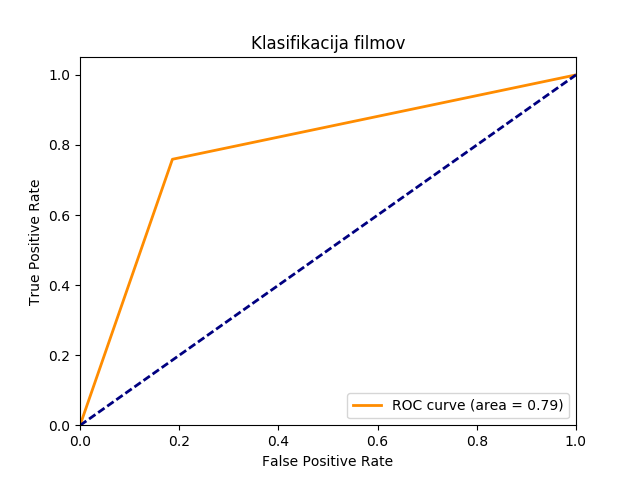
\includegraphics[scale=0.8]{slike/klasifikacija.png}
		\caption{Na grafu je predstavljena ROC krivulja in ploščina pod krivuljo. Osi predstavljata senzitivnost - True Positive Rate in druga os predstavlja False Positive Rate ki je 1-senzitivnost}
		\label{slika 3}
	\end{center}
\end{figure}

\begin{figure}[!htb]
	\begin{center}
		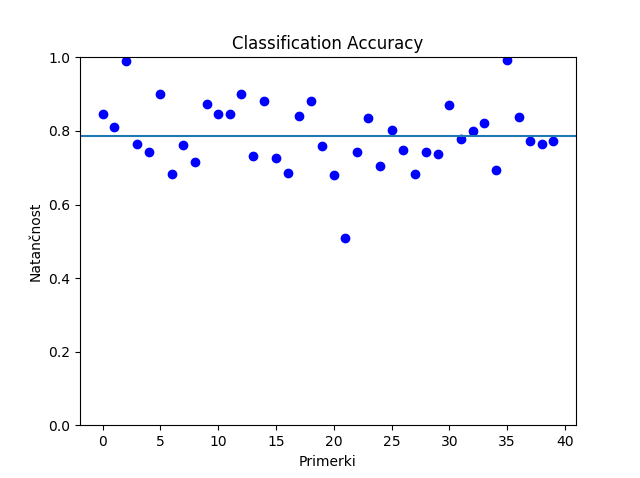
\includegraphics[scale=0.8]{slike/klasifikacija_1.png}
		\caption{Na grafu so označeni rezultati klasifikacijske točnosti za posamezen model. Večinski klasifikator znaša 0.61}
		\label{slika 4}
	\end{center}
\end{figure}

\end{document}
